\section{phase$\_$1}
	\begin{itemize}
	\item	
	第一关的汇编代码如下:
	\begin{figure}[h]
		\centering
			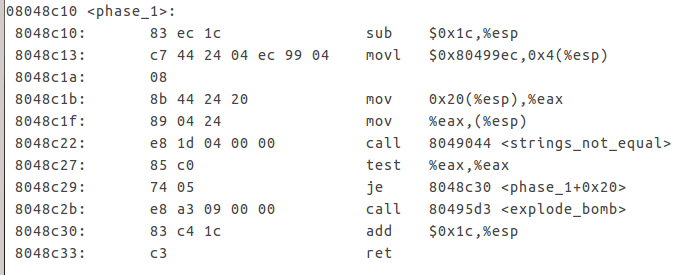
\includegraphics[scale=0.77]{images/phase_1.png}
	\end{figure}

	\item	
	这个函数较短,分析发现,它调用了一个名为\textbf{strings$\_$not$\_$equal}函数。
	
	分析\textbf{strings$\_$not$\_$equal}这个函数,发现它实现这样一个功能:
	
	比较两个字符串,相等返回0,不相等返回1
	
	\item
	分析call之后的程序,发现如果返回值(即$\%eax$)不为0的话,会调用\textbf{explode$\_$bomb}函数,炸弹会被引爆。因此,我们输入的字符串应该与某个字符串相同。
	
	\item
	这样,破解phase$\_$1的方法就很清晰了:

		\begin{center}
			\textbf{输入存在地址0x80499ec中的字符串}
		\end{center}

	\item
	于是现在的问题是找出存放在地址0x80499ec中的字符串。
	
	从调用strings$\_$not$\_$equal的语句向上看:
	\begin{figure}[h]
		\centering
			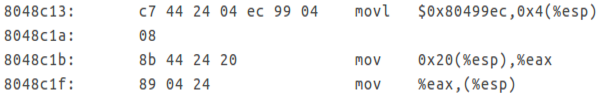
\includegraphics[scale=0.77]{images/phase_1_part_0.png}	
	\end{figure}
	
	这表示,这个函数的两个参数,一个是程序自身地址\textbf{0x80499ec},另一个\textbf{0x20(\%esp)}就是我们的输入参数。
	
	\item
	我们首先需要知道\textbf{0x80499ec}地址里存放的数据。于是使用\textbf{gdb},输入命令\textbf{p (char *) 0x80499ec},查看它存放的数据:
	\begin{figure}[h]
		\centering
			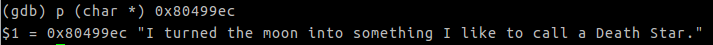
\includegraphics[scale=0.7]{images/phase_1_part_1.png};
	\end{figure}
	
	\item
	第一关的答案水落石出:输入\textbf{I turned the moon into something I like to call a Death Star.},顺利过关。
	\end{itemize}
	
	\begin{figure}[h]
		\centering
			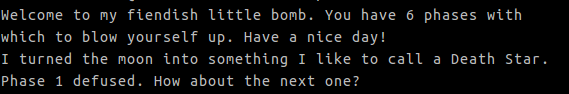
\includegraphics[scale=0.8]{images/phase_1_success.png};
	\end{figure}
	
	主要复习知识点:\textbf{常量的存储、函数的参数传递}
	